\documentclass[12pt]{article}

% set margins and spacing
\addtolength{\textwidth}{1.3in}
\addtolength{\oddsidemargin}{-.65in} %left margin
\addtolength{\evensidemargin}{-.65in}
\setlength{\textheight}{9in}
\setlength{\topmargin}{-.5in}
\setlength{\headheight}{0.0in}
\setlength{\footskip}{.375in}
\renewcommand{\baselinestretch}{1.0}
\linespread{1.0}

% load miscellaneous packages
\usepackage{csquotes}
\usepackage[american]{babel}
\usepackage[usenames,dvipsnames]{color}
\usepackage{graphicx,amsbsy,amssymb, amsmath, amsthm, MnSymbol,bbding,times, verbatim,bm,pifont,pdfsync,setspace,natbib}

% enable hyperlinks and table of contents
\usepackage[pdftex,
bookmarks=true,
bookmarksnumbered=false,
pdfview=fitH,
bookmarksopen=true,hyperfootnotes=false]{hyperref}



\begin{document}
\title{Taxes and Tariffs}
% add a fourth name if you have four team members; fill in at least first names below
\author{Dylan Thomas\thanks{Syracuse University, Economics Department. Email: economics@syr.edu } \and Kathryn Sarrge\thanks{} \and Umar Bilgrammi\thanks{}}
\date{\vskip-.1in \today}
\maketitle

\vskip.3in

\section{Research Question} \label{sec:question}

Are national commodity tax rates (VAT or sales tax depending on the country) and tariffs correlated in the data in developing countries? Do countries engage in complementary, or substitute strategies?

\section{Data Overview} \label{sec:literature}

We used two separate datasets from the World Integrated Trade Solutions website. The first dataset provides information on taxes on international trade while the second dataset gives us information on taxes on goods and services.

\subsection{Data Set 1: Taxes on international trade}
\begin{itemize}
  \item Source: World Integrated Trade Solution
  \item International trade data from developing countries given as a percent of revenue. The data is reported on a per year basis.
    \begin{itemize}
        \item 1988 - 2022
        \item Observations on developing countries and how they have experienced different levels of tariffs on international trade based on the overall revenue of the country
    \end{itemize}
  \item Variables
    \begin{itemize}
        \item  Taxes on international trade (given as a percent of revenue)
    \end{itemize}
  \item 194 countries with one variable plus one variable for each of the statistical question
\end{itemize}

\subsection{Data Set 2: Taxes on Goods and Services}

\begin{itemize}
  \item Source: World Integrated Trade Solution
  \item International tax data from developing countries given as a percent of revenue. The data is reported on a per year basis. 
    \begin{itemize}
        \item Years: 1988 - 2021
        \item Observations on developing countries and how they have experienced different levels of taxes on goods and services based on the overall revenue of the country
    \end{itemize}
  \item Variables
    \begin{itemize}
        \item Taxes on Goods and Services (given as a percent of revenue)
    \end{itemize}
  \item 194 with one variable plus one variable per statistical question
\end{itemize}

\noindent

\section{Data Acquisition}
\label{sec:theory}

The data sets can be acquired through from the 
 \href{https://wits.worldbank.org/CountryProfile/en/Country/BY-COUNTRY/StartYear/1988/EndYear/2022/Indicator/GC-TAX-GSRV-VA-ZS}{World Integrated Trade Solution}  website. To get the data, we altered the indicator on the website allowing us to get our two different data sets. Specifically, we used the indicators Taxes on Goods and Services (percent of revenue) and Taxes on international trade (percent of revenue). We downloaded these datasets by clicking the download button on the table view tab located on the right hand side above the data. The data is currently being stored in an issue named Data Use Log in our repository. Once in the repo, navigate to the issues in the top left bar of the website. Click on issues and access the top issue which reads Data Log. The second post in the issues section which is titled 10/10/2024, that reads Links for 2 data sets has the data. Data set 1 correlates to the first link and Data set 2 correlates to the second link.

\noindent
\begin{itemize}

    \item \href{https://github.com/ecn310/course-project-taxes-tariffs/issues/6}{Taxes and Tariffs Data Repo}
\end{itemize}


\section{Data Manipulation}
\label{sec:data}

\begin{itemize}
    \item The data manipulation will take place in Stata. Initially, we imported the data for international trade and taxes on goods and services separately into stata, converting them from wide to long. Our data is now in the correct format of long, and we are working on combining these two datasets to allow for statistical analysis of the data.
    \item File Documentation: All file documentation will occur in an issue named \href{https://github.com/ecn310/course-project-taxes-tariffs/issues/6}{Data Use Log} in our repository. Any time the data is altered, it will be listed there as to what we have done and when we did it.
\end{itemize}

\section{Visual Data}
\label{sec:graphs}

\section{Linking Datasets}
\label{sec:discussion}

\begin{itemize}
    \item \href{https://wits.worldbank.org/CountryProfile/en/Country/BY-COUNTRY/StartYear/1988/EndYear/2022/Indicator/GC-TAX-INTT-RV-ZS}{Data Set 1 Link}

 \item \href{https://wits.worldbank.org/CountryProfile/en/country/by-country/startyear/LTST/endyear/LTST/indicator/GC-TAX-GSRV-RV-ZS}{}
 \item In terms of linking the data together, we will use the percent of revenue variable to link these two datasets. They both have this variable in the dataset which allows us to link them together. 
\end{itemize}

\section{Key Variables}
\label{sec:result}



Data Set 1: 
\begin{itemize}
 \item Tax on Int'l Trade percent of revenue (continuous and ratio)
\end{itemize}
Data Set 2: 
\begin{itemize}
    \item Tax on G and S percent of Revenue (continuous and ratio)
\end{itemize}
\section{Hypothesis}
\begin{itemize}
    \item Working Hypothesis: (in developing countries) If domestic tax revenue increases then tariff revenue decreases
    \item Null Hypothesis: There is no correlation between domestic tax revenue and tariff revenue (at a country level)
\end{itemize}


\begin{figure}
    \centering
    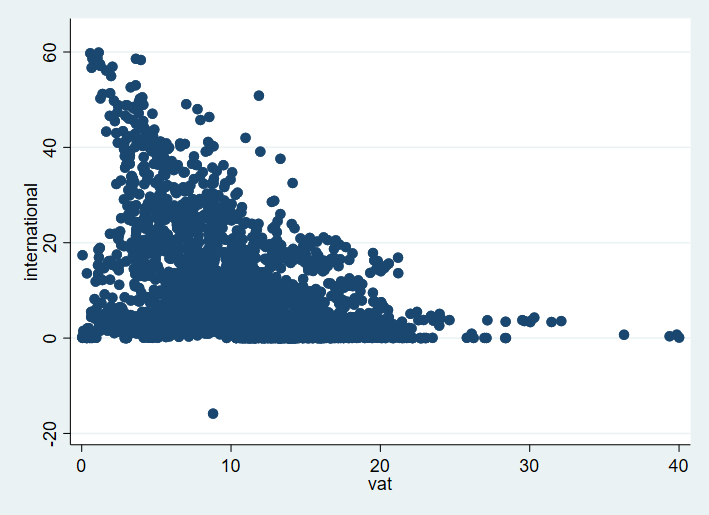
\includegraphics[width=0.5\linewidth]{mergedscatter.png}
    \caption{Merged Data Scatter Plot}
    \label{fig:enter-label}
\end{figure}



\begin{figure}
    \centering
    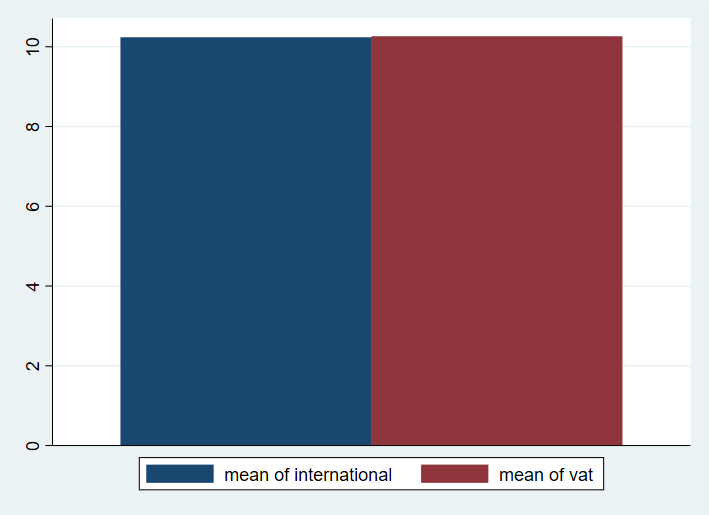
\includegraphics[width=0.5\linewidth]{mergedbar.png}
    \caption{Merged Data Mean Bar Graph}
    \label{fig:enter-label}
\end{figure}
\begin{figure}
    \centering
    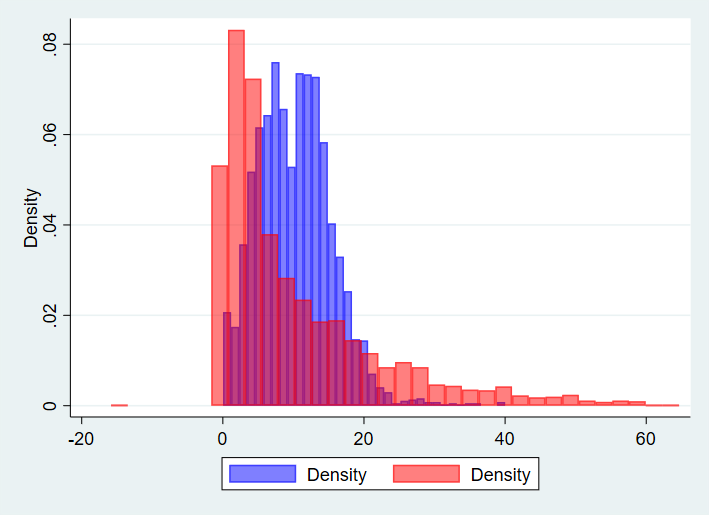
\includegraphics[width=0.5\linewidth]{.github/mergedhistogram.png}
    \caption{Merged Data Histogram}
    \label{fig:enter-label}
\end{figure}
\end{document}
